\graphicspath{{./chapitres/chapitre2/figures/}}
\setcounter{mtc}{2}
\chapter{Analyse\textcolor{white}{J}et\textcolor{white}{J}spécification\textcolor{white}{J}des\textcolor{white}{J}besoins}
\fancyhead[R]{\ungaramond\small\textbf{Chapitre\textcolor{white}{J}2:\textcolor{white}{J}Analyse\textcolor{white}{J}et\textcolor{white}{J}spécification\textcolor{white}{J}des\textcolor{white}{J}besoins}}
\minitoc
\newpage
\section*{Introduction}
Dans ce chapitre, nous allons analyser et identifier les besoins de ce projet. On va commencer par définir les acteurs de ce projet, identifier les besoins fonctionnels et non fonctionnels, réaliser le diagramme de cas d’utilisations global. Pour finir avec le backlog produit, la planification des sprints sans oublier l’architecture physique et logique de cette solution ainsi que les technologies et les logiciels utilisés pour aboutir au résultat voulu.


\section{Capture\textcolor{white}{J}des\textcolor{white}{J}besoins}
\subsection{Identification\textcolor{white}{J}des\textcolor{white}{J}acteurs}

Un acteur\textcolor{white}{J}est\textcolor{white}{J}une\textcolor{white}{J}entité\textcolor{white}{J}externe au\textcolor{white}{J}système. Il\textcolor{white}{J}représente\textcolor{white}{J}une\textcolor{white}{J}personne\textcolor{white}{J}ou\textcolor{white}{J}un\textcolor{white}{J}autre système\textcolor{white}{J}informatique s'attend\textcolor{white}{J}à\textcolor{white}{J}être\textcolor{white}{J}une\textcolor{white}{J}interface d'accès. Il\textcolor{white}{J}interagit\textcolor{white}{J}avec\textcolor{white}{J}le système en\textcolor{white}{J}envoyant\textcolor{white}{J}ou\textcolor{white}{J}en\textcolor{white}{J}recevant\textcolor{white}{J}des\textcolor{white}{J}messages
Par\textcolor{white}{J}ailleurs, notre\textcolor{white}{J}application\textcolor{white}{J}fera intervenir des acteurs primaires et des acteurs secondaires.

\textbf{Formulateur}: C’est la personne qui aura la main de créer et visualiser les simulations.

\newline \textbf{Marketeur}: C’est la personne qui aura la main de créer, visualiser et valider les simulations.


\subsection{Besoins\textcolor{white}{J}fonctionnels}
Le recueil des besoins fonctionnels est une phase primordiale dans le projet, elle détermine ce que le projet est censé faire et définir les cas d’utilisation pour chaque acteur. Notre solution contiendra ces différentes fonctionnalités :
\begin{itemize}
\begin{itemize}[label=--]
\item Un espace de création des simulations : L’utilisateur peut choisir le type des cheveux, la couleur de base ainsi que la couleur de la teinte puis générer la simulation. Cette dernière pourra être sauvegardée ou validée ou réinitialisée. L’utilisateur aura la possibilité de modifier les paramètres et régénérer la simulation.
\item Un espace de visualisation des simulations : Suite à la génération des simulations, l’utilisateur pourra comparer entre les images contenant la couleur de base et les images synthétisées et zoomer sur les images simulées.
\item Un espace de gestion des simulations : L’utilisateur pourra visualiser et filtrer la liste des simulations, rechercher une simulation et dupliquer une simulation.
\end{itemize}

\end{itemize}

\textcolor{white}{J} 
\subsection{Besoins\textcolor{white}{J}non\textcolor{white}{J}fonctionnels}
Il s’agit des besoins caractérisant le système en terme de performance et de qualité. Dans notre cas, les besoins non fonctionnels identifiés sont :

\begin{itemize}
\begin{itemize}[label=--]
\item\textcolor{white}{J} \textbf{La sécurité}\textcolor{white}{J}: Le flux de données doit être sécurisé pour garantir la confidentialité des informations. 
\item\textcolor{white}{J} \textbf{La rapidité de traitement}\textcolor{white}{J}:
Il\textcolor{white}{J}est\textcolor{white}{J}impérativement\textcolor{white}{J}nécessaire\textcolor{white}{J}que\textcolor{white}{J}la\textcolor{white}{J}durée d’exécution\textcolor{white}{J}des traitements\textcolor{white}{J}s’approche\textcolor{white}{J}le\textcolor{white}{J}plus\textcolor{white}{J}possible\textcolor{white}{J}du\textcolor{white}{J}temps\textcolor{white}{J}réel. 
\item\textcolor{white}{J} \textbf{La performance}\textcolor{white}{J}:
Répond à toutes les exigences des usagers d’une manière optimale. 
\item\textcolor{white}{J} \textbf{L’ergonomie}\textcolor{white}{J}:
La\textcolor{white}{J}plateforme\textcolor{white}{J}doit\textcolor{white}{J}être\textcolor{white}{J}facile\textcolor{white}{J}à\textcolor{white}{J}utiliser. En effet,\textcolor{white}{J}les\textcolor{white}{J}interfaces utilisateurs\textcolor{white}{J}doivent\textcolor{white}{J}être\textcolor{white}{J}conviviales\textcolor{white}{J}c’est-à-dire\textcolor{white}{J}simples,\textcolor{white}{J}ergonomiques\textcolor{white}{J}et\textcolor{white}{J}adaptées à\textcolor{white}{J}l’utilisateur.
\end{itemize}
\end{itemize}

\section{Backlog\textcolor{white}{J}du\textcolor{white}{J}produit}
\subsection{Les\textcolor{white}{J}histoires\textcolor{white}{J}du\textcolor{white}{J}Backlog\textcolor{white}{J}du\textcolor{white}{J}produit}
Le\textcolor{white}{J}tableau\textcolor{white}{J}\ref{tab:backlog}\textcolor{white}{J}présente Le backlog du produit de notre\textcolor{white}{J}application est\textcolor{white}{J}présenté si dessous.

\begin{center}
\textcolor{white}{J}\textcolor{white}{J}\textcolor{white}{J} \textcolor{white}{J} 

\begin{longtable}[!ht]{|m{1cm}|m{3cm}|m{1cm}|m{7cm}|m{1.5cm}|c|}
\hline
\textbf{id features} & \textbf{features} & \textbf{id story} & \textbf{User Story} & \textbf{Priorité}\\
\hline
1 & Création des simulations & 1.1 & En tant qu’utilisateur je souhaite choisir la couleur de la teinte. & 100\\
\cline{3-5}
&  & 1.2 & En tant qu’utilisateur je souhaite recevoir les images synthétisées en temps  réel. & 100\\
\cline{3-5}
&  & 1.3 & En tant qu’utilisateur je souhaite sauvegarder la session. & 80\\
\hline
2 & Visualisation des simulations & 2.1 & En tant qu’utilisateur je souhaite comparer entre les images synthétisées et les images de base. & 100\\
\cline{3-5}
&  & 2.2 & En tant qu’utilisateur je souhaite effectuer un zoom sur l’image synthétisée. & 100\\


\hline
3 & Gestion des simulations  & 3.1 & En tant qu’utilisateur je souhaite visualiser la liste des simulations. & 100\\
\cline{3-5}
&  & 3.2 & En tant qu’utilisateur je souhaite rechercher une simulation . & 100\\
\cline{3-5}
&  & 3.3 & En tant qu’utilisateur je souhaite filtrer la liste des simulations par état (validée et non validée). & 100\\

\hline
\caption{Product Backlog}
\label{tab:backlog}
\end{longtable}

\end{center}

Le backlog produit représenté dans la figure nous permet de définir dans chaque fonctionnalité les user stories, leurs identifiants et leurs priorités selon la difficulté de chaque tâche à faire au cours du développement de l’application.

\subsection{Planification\textcolor{white}{J}des\textcolor{white}{J}sprints}
Le\textcolor{white}{J}projet\textcolor{white}{J}s'est\textcolor{white}{J} déroulé\textcolor{white}{J} pendant\textcolor{white}{J} six\textcolor{white}{J} mois\textcolor{white}{J} et\textcolor{white}{J} s'est\textcolor{white}{J} étendu\textcolor{white}{J} sur\textcolor{white}{J} la\textcolor{white}{J} période\textcolor{white}{J} entre\textcolor{white}{J} le\textcolor{white}{J} 01\textcolor{white}{J} Décembre\textcolor{white}{J} 2021\textcolor{white}{J} et\textcolor{white}{J} le\textcolor{white}{J} 30\textcolor{white}{J} Avril\textcolor{white}{J} 2022.

\begin{table}[h!]
\center
\begin{tabular}[b]{|m{3cm}|m{3cm}|m{3cm}|m{3cm}|}
\hline
\rowcolor{white}
Sprint 0 & Sprint 1 & Sprint 2 & Sprint 3 \\
\hline
Compréhension du périmètre fonctionnel et étude des besoins clients fonctionnels et non fonctionnels & mise en place du protocole de communication avec le moteur graphique & Développement de la partie backend & Développement de la partie frontend et déploiement de la solution \\
\hline
Du 1 Décembre au 3 Janvier  & Du 4 Janvier au 29 Janvier & Du 31 Janvier au 31 Mars & Du 1 Avril au 15 Avril \\
\hline
\end{tabular}
\caption{Planification\textcolor{white}{J}des\textcolor{white}{J}sprints}
\label{tab:tab-s}
\end{table}

\newpage
\section{Analyse}
\subsection{Modélisation\textcolor{white}{J}de\textcolor{white}{J}cas\textcolor{white}{J}d'utilisation}
En\textcolor{white}{J}UML, pour\textcolor{white}{J}avoir\textcolor{white}{J}une\textcolor{white}{J}capture sur les fonctionnalités\textcolor{white}{J}du\textcolor{white}{J}système, on utilise le diagramme de cas d’utilisation. Ce diagramme est représenté par la figure \ref{fig:usecaseGlob}.


\begin{figure}[!ht]
\centering
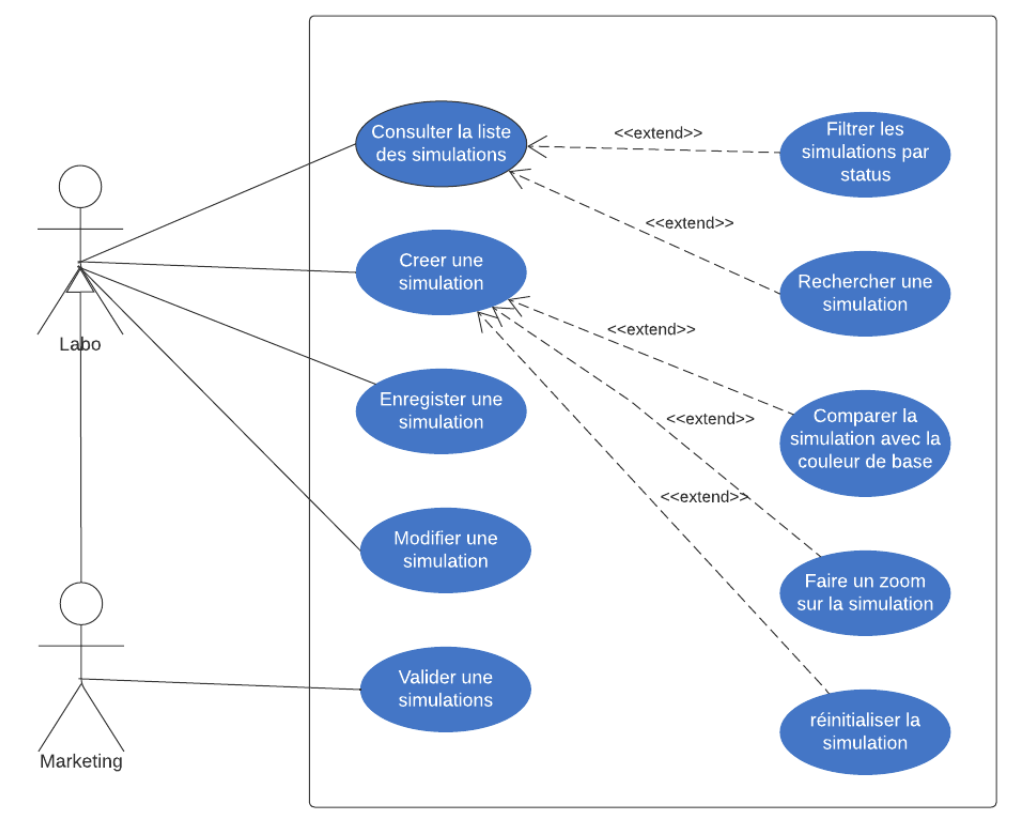
\includegraphics[width=1\textwidth,angle=00]{chapitres/chapitre2/figures/diagUseCaseGen.png}
\caption{Diagramme\textcolor{white}{J}de\textcolor{white}{J}cas\textcolor{white}{J}d'utilisation\textcolor{white}{J}global}
\label{fig:usecaseGlob}
\end{figure}

Le Formulateur peut consulter la listes des simulations où il a le choix de filtrer par status et rechercher une simulation.Il peut egalement creer une simulation en specifiant le type de cheveux ,la couleur de base et la couleur personnalisée ensuite il aura les differents perspectives de la simulation.Il peut comparer la simulation avec la couleur de base,effectuer un zoom sur une perspective ou reinitialiser la simulation.
Apres avoir simuler une couleur de cheveux,le formulateur peut la modifier ou l'enregistrer.
Finalement,Le marketeur peut valider une simulation.

\newpage
\subsection{Diagramme\textcolor{white}{J}de\textcolor{white}{J}classe\textcolor{white}{J}d'analyse}
la figure \ref{fig:usecasegenerale} représente le diagramme de classe d'analyse globale de notre projet.
\textcolor{white}{J} \begin{figure}[!ht]
\centering
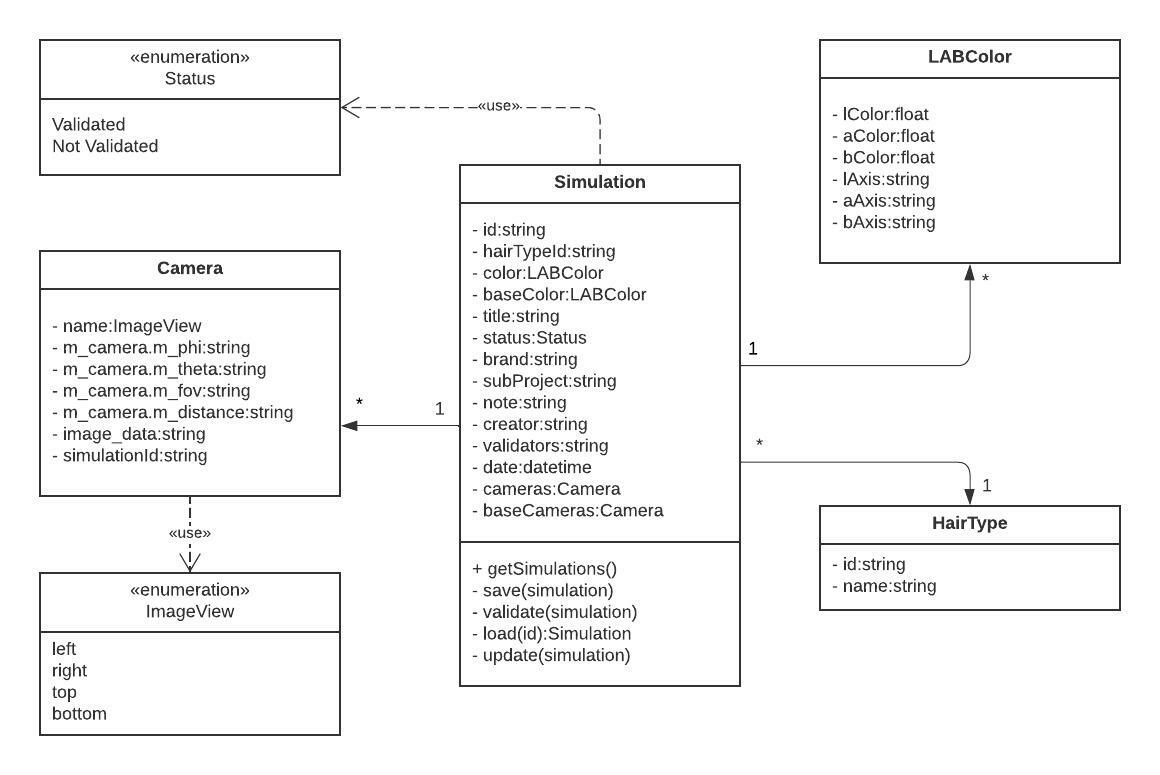
\includegraphics[width=1\textwidth,angle=00]{chapitres/chapitre2/figures/Diagramme de classe global.jpeg}
\caption{Diagramme\textcolor{white}{J}de\textcolor{white}{J}classe\textcolor{white}{J}d'analyse\textcolor{white}{J}global}
\label{fig:usecasegenerale}
\end{figure}
Une simulation est caracterisée par un identifiant unique,un type de cheveux,une couleur de base et une couleur personnalisée de type LABColor,un titre,un projet,une marque,une description,un createur, la liste des validateurs,la date de creation et la liste des differents perspetives de la couleur simulées et la couleur de base.


\newpage
\subsection{Environnement\textcolor{white}{J}logiciel}
Dans\textcolor{white}{J}cette \textcolor{white}{J}partie, \textcolor{white}{J}on \textcolor{white}{J}va \textcolor{white}{J}présenter \textcolor{white}{J}les \textcolor{white}{J}différents \textcolor{white}{J}Framework, \textcolor{white}{J}technologies, \textcolor{white}{J}outils, \textcolor{white}{J}et \textcolor{white}{J}configurations \textcolor{white}{J}nécessaires \textcolor{white}{J}pour \textcolor{white}{J}l’implémentation \textcolor{white}{J}de \textcolor{white}{J}l’application.

\subsubsection*{.NET Core [2]}
ASP.NET Core est une infrastructure multiplateforme, haute performance et open source permettant de créer des applications modernes, compatibles avec le cloud et connectées à Internet. Avec ASP.NET Core, nous aurons la possibilité de créer des applications web et des services et des back-ends mobiles et déployer nos solutions dans le cloud ou localement.



\subsubsection*{React Js[3]}
ReactJS est une bibliothèque JavaScript déclarative, efficace et flexible permettant de créer des interfaces utilisateur (UI). Ce Framework permet de composer des interfaces utilisateur complexes à partir de petits morceaux de code isolés appelés « composants ».


\subsubsection*{Visual Studio [4]}
Visual Studio IDE (Integrated Development Environment) complet idéal pour les développeurs .NET et C++ sur Windows. Entièrement rempli d’un bon ensemble d’outils et de fonctionnalités permettant d’élever et d’améliorer chaque étape du développement de logiciels. 



\subsubsection*{GitLab[5]}
GitLab est un logiciel libre de forge basé sur git et un système de suivi des bugs, l’intégration continue et la livraison continue. Le logiciel est utilisé par plusieurs grandes entreprises informatiques, dont L’Oréal.




\subsubsection*{ShareLaTeX[6]}
ShareLaTeX\textcolor{white}{J} est\textcolor{white}{J} un\textcolor{white}{J} éditeur\textcolor{white}{J} LaTeX\textcolor{white}{J} en\textcolor{white}{J} ligne,\textcolor{white}{J} collaboratif,\textcolor{white}{J} en\textcolor{white}{J} temps\textcolor{white}{J} réel\textcolor{white}{J} et\textcolor{white}{J} compileur\textcolor{white}{J} PDF.\textcolor{white}{J} Par\textcolor{white}{J} ailleurs,\textcolor{white}{J} ShareLaTeX\textcolor{white}{J} fut\textcolor{white}{J} libéré\textcolor{white}{J} en\textcolor{white}{J} février\textcolor{white}{J} 2014.\textcolor{white}{J} Le\textcolor{white}{J} 20\textcolor{white}{J} Juillet\textcolor{white}{J} 2017,\textcolor{white}{J} ShareLatex\textcolor{white}{J} a\textcolor{white}{J} été\textcolor{white}{J} racheté\textcolor{white}{J} par\textcolor{white}{J} overleaf5\textcolor{white}{J} qui\textcolor{white}{J} a\textcolor{white}{J} réuni\textcolor{white}{J} les\textcolor{white}{J} services\textcolor{white}{J} d'overleaf\textcolor{white}{J} et\textcolor{white}{J} de\textcolor{white}{J} Sharelatex\textcolor{white}{J} sur\textcolor{white}{J} une\textcolor{white}{J} seule\textcolor{white}{J} plateforme\textcolor{white}{J} .\textcolor{white}{J} La\textcolor{white}{J} fusion\textcolor{white}{J} des\textcolor{white}{J} deux\textcolor{white}{J} services\textcolor{white}{J} au\textcolor{white}{J} sein\textcolor{white}{J} de\textcolor{white}{J} overleaf\textcolor{white}{J} v2\textcolor{white}{J} a\textcolor{white}{J} été\textcolor{white}{J} effectué\textcolor{white}{J} au\textcolor{white}{J} mois\textcolor{white}{J} de\textcolor{white}{J} septembre\textcolor{white}{J} 2018. \\



\subsubsection*{VsCode[7]}
Visual Studio Code est un Éditeur de code source autonome qui est le meilleur choix le développement web, avec des extensions pour prendre en charge à peu près n’importe quel langage de programmation.




\section{Spécification\textcolor{white}{J}Architecturale}
\subsection{Architecture\textcolor{white}{J}logique}
L’architecture logique d’une application informatique c’est l’organisation des composants logiques de chaque solution. 

\subsubsection{Architecture\textcolor{white}{J}Back-end}
La partie Backend interagit avec la partie présentation ou bien frontend en la fournissant par les métiers implémentés. Elle est divisée en 3 couches : La première c’est la couche modèle qui contient les documents connectés directement avec notre base de données. La deuxième est la couche services, c’est l’intermédiaire entre les autres couches en leur fournissant les services et les métiers de l’application. La troisième est la couche Controller, elle assurer la communication entre la partie serveur et client en envoyant des requêtes HTTP définis par le Rest API. Le client communiquera aussi avec le serveur avec le bus de communication instantané Web Socket.

\begin{figure}[!ht]
\centering
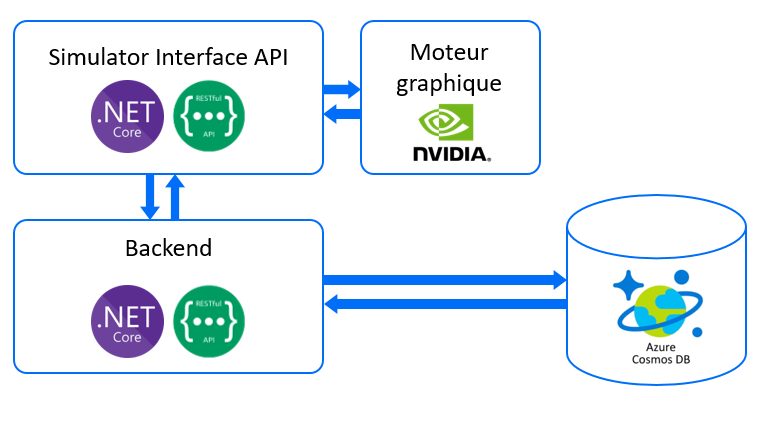
\includegraphics[width=0.8\textwidth,angle=00]{chapitres/chapitre2/figures/ArchLog-B.png}
\caption{Architecture\textcolor{white}{J}logique\textcolor{white}{J}des\textcolor{white}{J}serveur\textcolor{white}{J}d'application}
\label{fig:archb}
\end{figure}

\newpage
\subsubsection{Architecture\textcolor{white}{J}Front-end}
L’architecture logique d’une application informatique c’est l’organisation des composants logiques de chaque solution.
\begin{figure}[!ht]
\centering
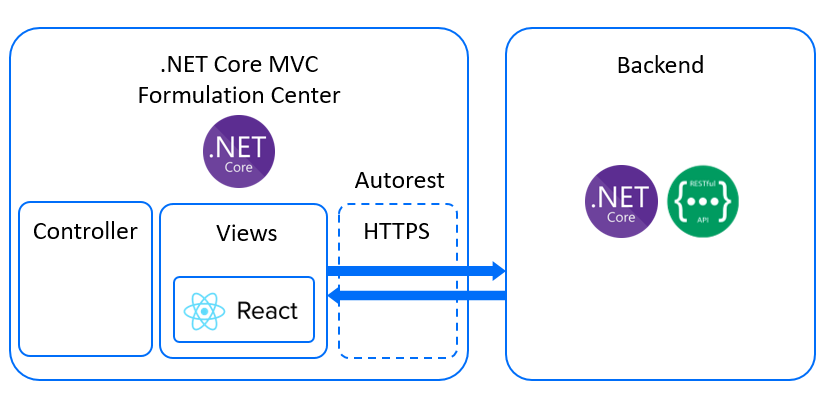
\includegraphics[width=0.8\textwidth,angle=00]{chapitres/chapitre2/figures/ArchLog-F.png}
\caption{Architecture\textcolor{white}{J}logique\textcolor{white}{J}Front-end}
\label{fig:logiqueFront}
\end{figure}

\subsection{Architecture\textcolor{white}{J}physique}
L’architecture\textcolor{white}{J}physique nous permet de décrire les composants matériels de l’application, avant de commencer la conception et le développement de l’application nous devons préparer cette architecture. Elle est décrite dans la figure \ref{fig:physique} ci-dessous.

\begin{figure}[!ht]
\centering
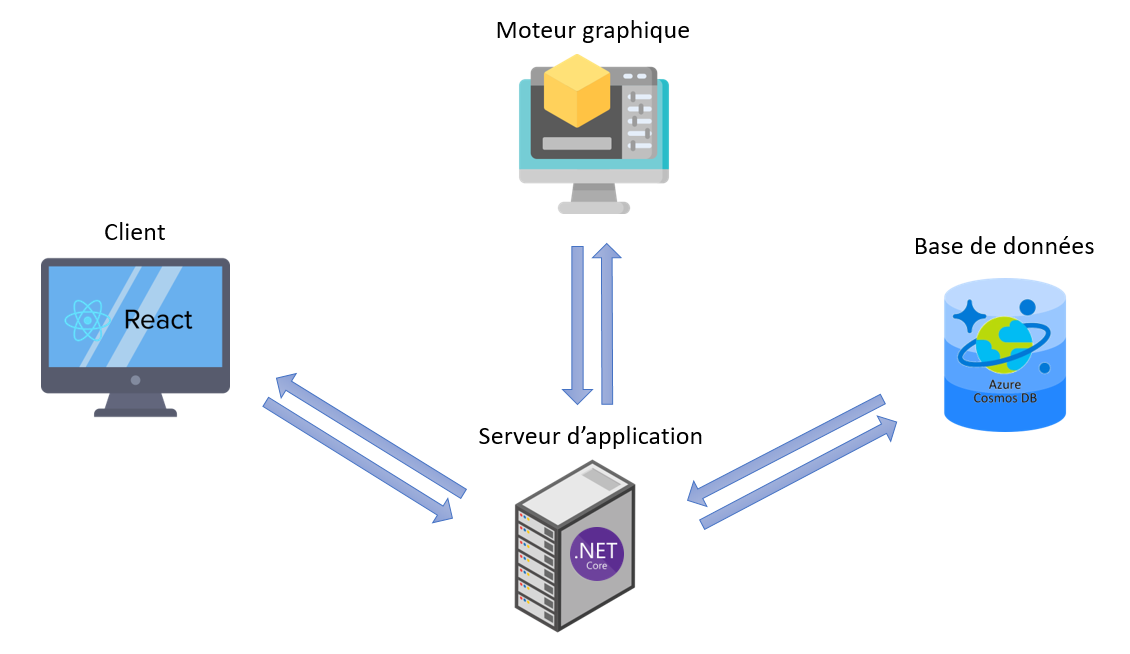
\includegraphics[width=0.8\textwidth,angle=00]{chapitres/chapitre2/figures/ArchPhy.png}
\caption{Architecture physique\textcolor{white}{J}de\textcolor{white}{J}notre\textcolor{white}{J}application}
\label{fig:physique}
\end{figure}

\begin{figure}[!ht]
\centering
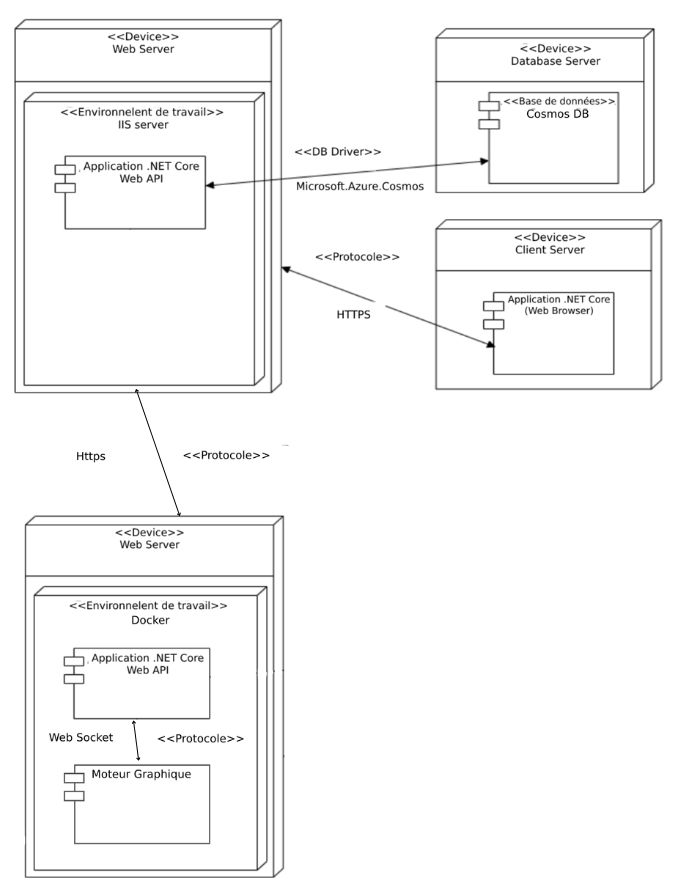
\includegraphics[width=0.8\textwidth,angle=00]{chapitres/chapitre2/figures/architecture physique.png}
\caption{Diagramme de deploiement de\textcolor{white}{J}notre\textcolor{white}{J}application}
\label{fig:physique}
\end{figure}


\section{Environnement\textcolor{white}{J}de\textcolor{white}{J}travail}
Afin de réaliser le projet, la société nous a fourni un ordinateur HP et un VDI Citrix VDI (infrastructure de postes de travail virtuels) et DaaS (Desktop-as-a-Service). C’est une forme de virtualisation de postes qui prend en charge les utilisateurs mobiles et l’accès distant.
Le VDI améliore la sécurité par rapport à une exécution locale. Toutes les données d’une connexion VDI résident sur le serveur, pas sur l’appareil. En cas de vol d’un point de terminaison, il n’y a donc rien à exfiltrer de son stockage local. En outre, l’environnement VDI est entièrement contrôlé de façon centralisée depuis un Datacenter L’Oréal.
Les solutions de bureaux virtuels soutiennent la mobilité et l’accès distant, et permettent au service IT de délivrer des postes de travail de façon sécurisée.

\section*{Conclusion}
Tous les besoins fonctionnels et non fonctionnels ont été traité par ce deuxième chapitre et cela a été fait par la présentation du diagramme de cas d’utilisation global ainsi que le backlog produit ce qui a engendré une planification optimale des différents sprints du projet. Ce chapitre nous a permis de mettre l’accent sur l’architecture physique et logique et aussi de spécifier les technologies et les outils auxquels nous avons eu recours.